\documentclass{standalone}
\usepackage{tikz}
\usetikzlibrary{patterns, positioning}


\begin{document}
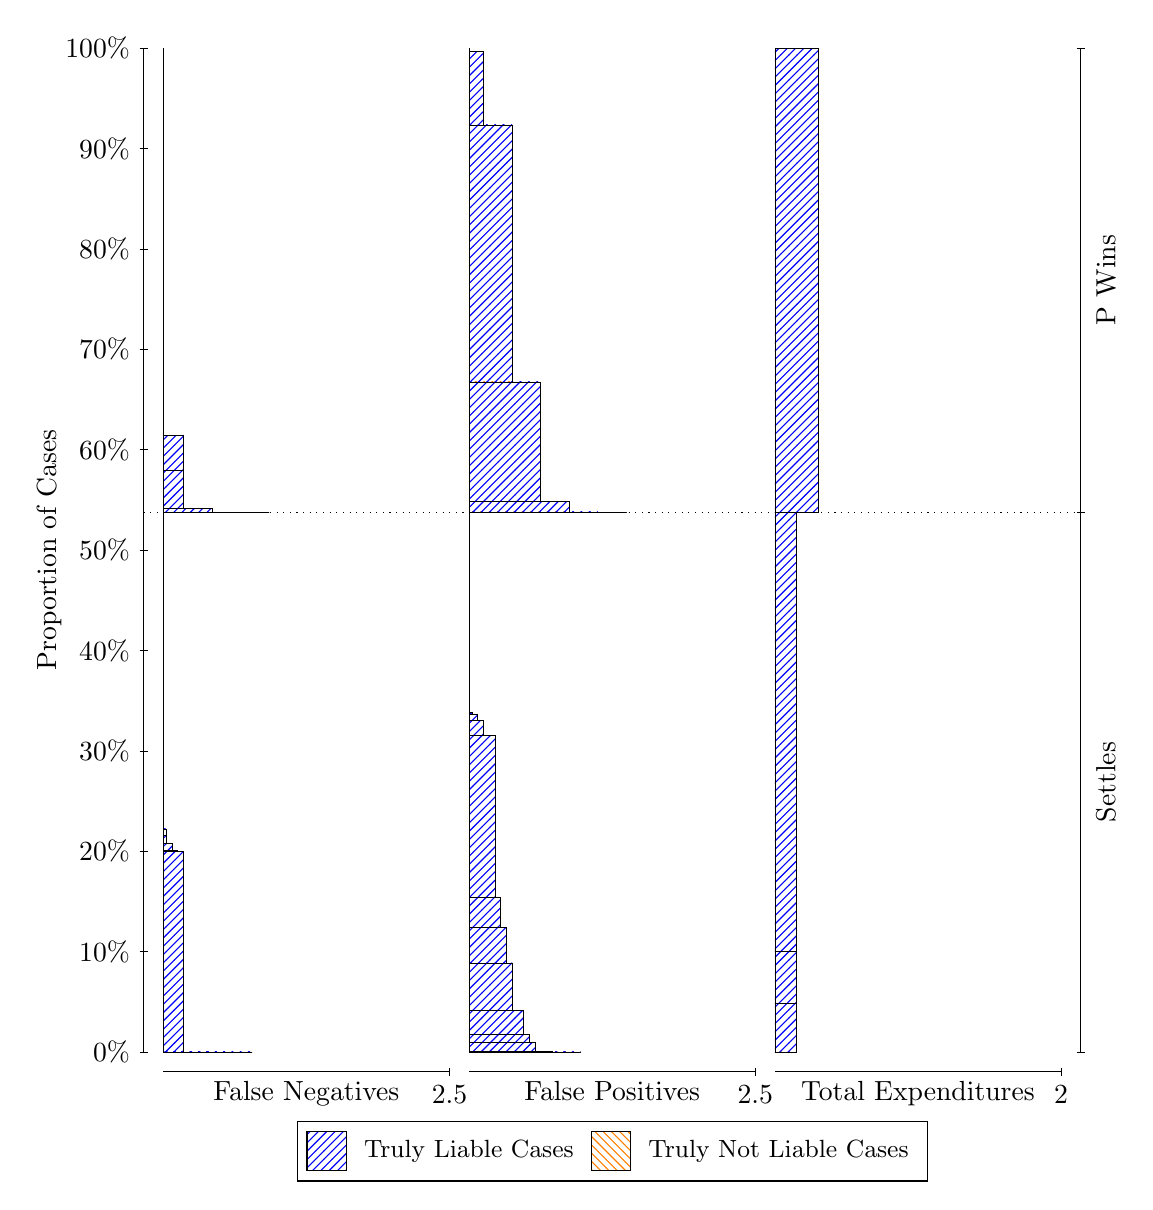
\begin{tikzpicture}
\draw[black, very thin] (1.5,1.75) -- (1.5,14.5);
\node[rotate=90, text=black, anchor=center] at (0.3, 8.125) {Proportion of Cases};
\draw[black, very thin] (1.45,1.75) -- (1.55,1.75);
\node[text=black, anchor=east] at (1.45, 1.75) {0\%};
\draw[black, very thin] (1.45,3.025) -- (1.55,3.025);
\node[text=black, anchor=east] at (1.45, 3.025) {10\%};
\draw[black, very thin] (1.45,4.3) -- (1.55,4.3);
\node[text=black, anchor=east] at (1.45, 4.3) {20\%};
\draw[black, very thin] (1.45,5.575) -- (1.55,5.575);
\node[text=black, anchor=east] at (1.45, 5.575) {30\%};
\draw[black, very thin] (1.45,6.85) -- (1.55,6.85);
\node[text=black, anchor=east] at (1.45, 6.85) {40\%};
\draw[black, very thin] (1.45,8.125) -- (1.55,8.125);
\node[text=black, anchor=east] at (1.45, 8.125) {50\%};
\draw[black, very thin] (1.45,9.4) -- (1.55,9.4);
\node[text=black, anchor=east] at (1.45, 9.4) {60\%};
\draw[black, very thin] (1.45,10.675) -- (1.55,10.675);
\node[text=black, anchor=east] at (1.45, 10.675) {70\%};
\draw[black, very thin] (1.45,11.95) -- (1.55,11.95);
\node[text=black, anchor=east] at (1.45, 11.95) {80\%};
\draw[black, very thin] (1.45,13.225) -- (1.55,13.225);
\node[text=black, anchor=east] at (1.45, 13.225) {90\%};
\draw[black, very thin] (1.45,14.5) -- (1.55,14.5);
\node[text=black, anchor=east] at (1.45, 14.5) {100\%};

\draw[black, very thin] (13.4,1.75) -- (13.4,14.5);
\draw[black, very thin] (13.35,1.75) -- (13.45,1.75);
\node[anchor=west] at (13.35, 1.75) {};
\draw[black, very thin] (13.35,8.6067) -- (13.45,8.6067);
\node[anchor=west] at (13.35, 8.6067) {};
\draw[black, very thin] (13.35,14.5) -- (13.45,14.5);
\node[anchor=west] at (13.35, 14.5) {};

\draw[black, very thin, pattern color=blue, pattern=north east lines] (1.75,1.75) rectangle (2.8763,1.75);
\draw[black, very thin, pattern color=blue, pattern=north east lines] (1.75,1.75) rectangle (2.5857,1.75);
\draw[black, very thin, pattern color=blue, pattern=north east lines] (1.75,1.75) rectangle (2.513,1.75);
\draw[black, very thin, pattern color=blue, pattern=north east lines] (1.75,1.75) rectangle (2.4403,1.75);
\draw[black, very thin, pattern color=blue, pattern=north east lines] (1.75,1.75) rectangle (2.295,1.75);
\draw[black, very thin, pattern color=blue, pattern=north east lines] (1.75,1.75) rectangle (2.2223,1.7501);
\draw[black, very thin, pattern color=blue, pattern=north east lines] (1.75,1.7501) rectangle (2.1497,1.7509);
\draw[black, very thin, pattern color=blue, pattern=north east lines] (1.75,1.7509) rectangle (2.1497,1.7519);
\draw[black, very thin, pattern color=blue, pattern=north east lines] (1.75,1.7519) rectangle (2.077,1.7519);
\draw[black, very thin, pattern color=blue, pattern=north east lines] (1.75,1.7519) rectangle (2.0043,4.2967);
\draw[black, very thin, pattern color=blue, pattern=north east lines] (1.75,4.2967) rectangle (1.9317,4.3134);
\draw[black, very thin, pattern color=blue, pattern=north east lines] (1.75,4.3134) rectangle (1.859,4.3983);
\draw[black, very thin, pattern color=blue, pattern=north east lines] (1.75,4.3983) rectangle (1.7863,4.4986);
\draw[black, very thin, pattern color=blue, pattern=north east lines] (1.75,4.4986) rectangle (1.7863,4.5838);
\draw[black, very thin, pattern color=orange, pattern=north west lines] (1.75,4.5838) rectangle (1.75,4.5838);
\draw[black, very thin, pattern color=blue, pattern=north east lines] (1.75,4.5838) rectangle (1.75,8.6067);
\draw[black, very thin, pattern color=blue, pattern=north east lines] (1.75,8.6067) rectangle (3.0943,8.6067);
\draw[black, very thin, pattern color=blue, pattern=north east lines] (1.75,8.6067) rectangle (2.731,8.6068);
\draw[black, very thin, pattern color=blue, pattern=north east lines] (1.75,8.6068) rectangle (2.3677,8.6537);
\draw[black, very thin, pattern color=blue, pattern=north east lines] (1.75,8.6537) rectangle (2.0043,9.1358);
\draw[black, very thin, pattern color=blue, pattern=north east lines] (1.75,9.1358) rectangle (2.0043,9.5813);
\draw[black, very thin, pattern color=orange, pattern=north west lines] (1.75,9.5813) rectangle (1.75,9.5813);
\draw[black, very thin, pattern color=blue, pattern=north east lines] (1.75,9.5813) rectangle (1.75,14.5);
\draw[black, very thin, pattern color=orange, pattern=north west lines] (5.6333,1.75) rectangle (7.0503,1.75);
\draw[black, very thin, pattern color=blue, pattern=north east lines] (5.6333,1.75) rectangle (7.0503,1.75);
\draw[black, very thin, pattern color=orange, pattern=north west lines] (5.6333,1.75) rectangle (6.905,1.75);
\draw[black, very thin, pattern color=blue, pattern=north east lines] (5.6333,1.75) rectangle (6.905,1.75);
\draw[black, very thin, pattern color=orange, pattern=north west lines] (5.6333,1.75) rectangle (6.7597,1.75);
\draw[black, very thin, pattern color=blue, pattern=north east lines] (5.6333,1.75) rectangle (6.7597,1.751);
\draw[black, very thin, pattern color=blue, pattern=north east lines] (5.6333,1.751) rectangle (6.687,1.7527);
\draw[black, very thin, pattern color=orange, pattern=north west lines] (5.6333,1.7527) rectangle (6.6143,1.7527);
\draw[black, very thin, pattern color=blue, pattern=north east lines] (5.6333,1.7527) rectangle (6.6143,1.7527);
\draw[black, very thin, pattern color=blue, pattern=north east lines] (5.6333,1.7527) rectangle (6.5417,1.7536);
\draw[black, very thin, pattern color=orange, pattern=north west lines] (5.6333,1.7536) rectangle (6.469,1.7536);
\draw[black, very thin, pattern color=blue, pattern=north east lines] (5.6333,1.7536) rectangle (6.469,1.8736);
\draw[black, very thin, pattern color=blue, pattern=north east lines] (5.6333,1.8736) rectangle (6.3963,1.9746);
\draw[black, very thin, pattern color=blue, pattern=north east lines] (5.6333,1.9746) rectangle (6.3237,2.2779);
\draw[black, very thin, pattern color=blue, pattern=north east lines] (5.6333,2.2779) rectangle (6.251,2.2781);
\draw[black, very thin, pattern color=orange, pattern=north west lines] (5.6333,2.2781) rectangle (6.1783,2.2781);
\draw[black, very thin, pattern color=blue, pattern=north east lines] (5.6333,2.2781) rectangle (6.1783,2.8805);
\draw[black, very thin, pattern color=blue, pattern=north east lines] (5.6333,2.8805) rectangle (6.1057,3.3315);
\draw[black, very thin, pattern color=blue, pattern=north east lines] (5.6333,3.3315) rectangle (6.033,3.7137);
\draw[black, very thin, pattern color=blue, pattern=north east lines] (5.6333,3.7137) rectangle (5.9603,5.7727);
\draw[black, very thin, pattern color=blue, pattern=north east lines] (5.6333,5.7727) rectangle (5.8877,5.7728);
\draw[black, very thin, pattern color=blue, pattern=north east lines] (5.6333,5.7728) rectangle (5.815,5.9583);
\draw[black, very thin, pattern color=blue, pattern=north east lines] (5.6333,5.9583) rectangle (5.7423,6.0433);
\draw[black, very thin, pattern color=blue, pattern=north east lines] (5.6333,6.0433) rectangle (5.6697,6.06);
\draw[black, very thin, pattern color=blue, pattern=north east lines] (5.6333,6.06) rectangle (5.6333,8.6067);
\draw[black, very thin, pattern color=orange, pattern=north west lines] (5.6333,8.6067) rectangle (7.6317,8.6067);
\draw[black, very thin, pattern color=blue, pattern=north east lines] (5.6333,8.6067) rectangle (7.6317,8.6067);
\draw[black, very thin, pattern color=orange, pattern=north west lines] (5.6333,8.6067) rectangle (7.2683,8.6067);
\draw[black, very thin, pattern color=blue, pattern=north east lines] (5.6333,8.6067) rectangle (7.2683,8.6086);
\draw[black, very thin, pattern color=orange, pattern=north west lines] (5.6333,8.6086) rectangle (6.905,8.6086);
\draw[black, very thin, pattern color=blue, pattern=north east lines] (5.6333,8.6086) rectangle (6.905,8.7468);
\draw[black, very thin, pattern color=orange, pattern=north west lines] (5.6333,8.7468) rectangle (6.5417,8.7468);
\draw[black, very thin, pattern color=blue, pattern=north east lines] (5.6333,8.7468) rectangle (6.5417,10.261);
\draw[black, very thin, pattern color=orange, pattern=north west lines] (5.6333,10.261) rectangle (6.1783,10.261);
\draw[black, very thin, pattern color=blue, pattern=north east lines] (5.6333,10.261) rectangle (6.1783,13.525);
\draw[black, very thin, pattern color=blue, pattern=north east lines] (5.6333,13.525) rectangle (5.815,14.453);
\draw[black, very thin, pattern color=blue, pattern=north east lines] (5.6333,14.453) rectangle (5.6333,14.5);
\draw[black, very thin, pattern color=orange, pattern=north west lines] (9.5167,1.75) rectangle (9.7892,1.75);
\draw[black, very thin, pattern color=blue, pattern=north east lines] (9.5167,1.75) rectangle (9.7892,2.3683);
\draw[black, very thin, pattern color=orange, pattern=north west lines] (9.5167,2.3683) rectangle (9.7892,2.3683);
\draw[black, very thin, pattern color=blue, pattern=north east lines] (9.5167,2.3683) rectangle (9.7892,3.0244);
\draw[black, very thin, pattern color=orange, pattern=north west lines] (9.5167,3.0244) rectangle (9.7892,3.0244);
\draw[black, very thin, pattern color=blue, pattern=north east lines] (9.5167,3.0244) rectangle (9.7892,8.6067);
\draw[black, very thin, pattern color=orange, pattern=north west lines] (9.5167,8.6067) rectangle (10.062,8.6067);
\draw[black, very thin, pattern color=blue, pattern=north east lines] (9.5167,8.6067) rectangle (10.062,14.5);
\draw[black, dotted] (1.5,8.6067) -- (13.4,8.6067);
\draw[black, very thin] (1.75,1.5) -- (5.3833,1.5);
\node[text=black, anchor=north] at (3.5667, 1.5) {False Negatives};
\draw[black, very thin] (5.3833,1.45) -- (5.3833,1.55);
\node[text=black, anchor=north] at (5.3833, 1.45) {2.5};

\draw[black, very thin] (5.6333,1.5) -- (9.2667,1.5);
\node[text=black, anchor=north] at (7.45, 1.5) {False Positives};
\draw[black, very thin] (9.2667,1.45) -- (9.2667,1.55);
\node[text=black, anchor=north] at (9.2667, 1.45) {2.5};

\draw[black, very thin] (9.5167,1.5) -- (13.15,1.5);
\node[text=black, anchor=north] at (11.333, 1.5) {Total Expenditures};
\draw[black, very thin] (13.15,1.45) -- (13.15,1.55);
\node[text=black, anchor=north] at (13.15, 1.45) {2};

\node[text=black, centered, rotate=90] at (13.72, 5.1783) {Settles};
\node[text=black, centered, rotate=90] at (13.72, 11.553) {P Wins};

\draw (7.449999999999999,1.5) node[draw=none] (baseCoordinate) {};
\begin{scope}[align=center]
        \matrix[scale=0.5, draw=black, below=0.5cm of baseCoordinate, nodes={draw}, column sep=0.1cm]{
            \node[rectangle, draw, minimum width=0.5cm, minimum height=0.5cm, pattern color=blue, pattern=north east lines] {}; &
            \node[draw=none, font=\small, text=black] (B) {Truly Liable Cases}; &
            \node[rectangle, draw, minimum width=0.5cm, minimum height=0.5cm, pattern color=orange, pattern=north west lines] {}; &
            \node[draw=none, font=\small, text=black] (B) {Truly Not Liable Cases}; \\
            };
\end{scope}

\end{tikzpicture}
\end{document}